   \documentclass[spanish]{article}
\usepackage{babel}
\usepackage[utf8]{inputenc}
\usepackage{graphicx}

\begin{document}
\begin{titlepage}

\centering
	\vspace{1cm}
	{\scshape\LARGE Instituto Politécnico Nacional \par}
	\vspace{0.7cm}
	{\scshape\Large Escuela Superior de Cómputo\par}
	\vspace{1.5cm}
	{\huge\bfseries Automata para reconocimiento de cadenas con terminación ing\par}
	\vspace{2cm}
	{\Large\itshape Mercado Rogel Martin Isauro\par}
	\vspace{0.7cm}
	{\large 2014090449\par}
	\vspace{0.7cm}
	{\large Teoría computacional\par}
	\vspace{0.7cm}
	{\large 2CV1\par}
	\vfill
	%supervised by\par
	%Dr.~Mark \textsc{Brown}

	\vfill

% Bottom of the page
	{\large \today\par}
\end{titlepage}
Se pide realizar un automata que reconozca todas las palabras con terminación ing.\\
El automata tiene el siguiente diagrama de estados:\\
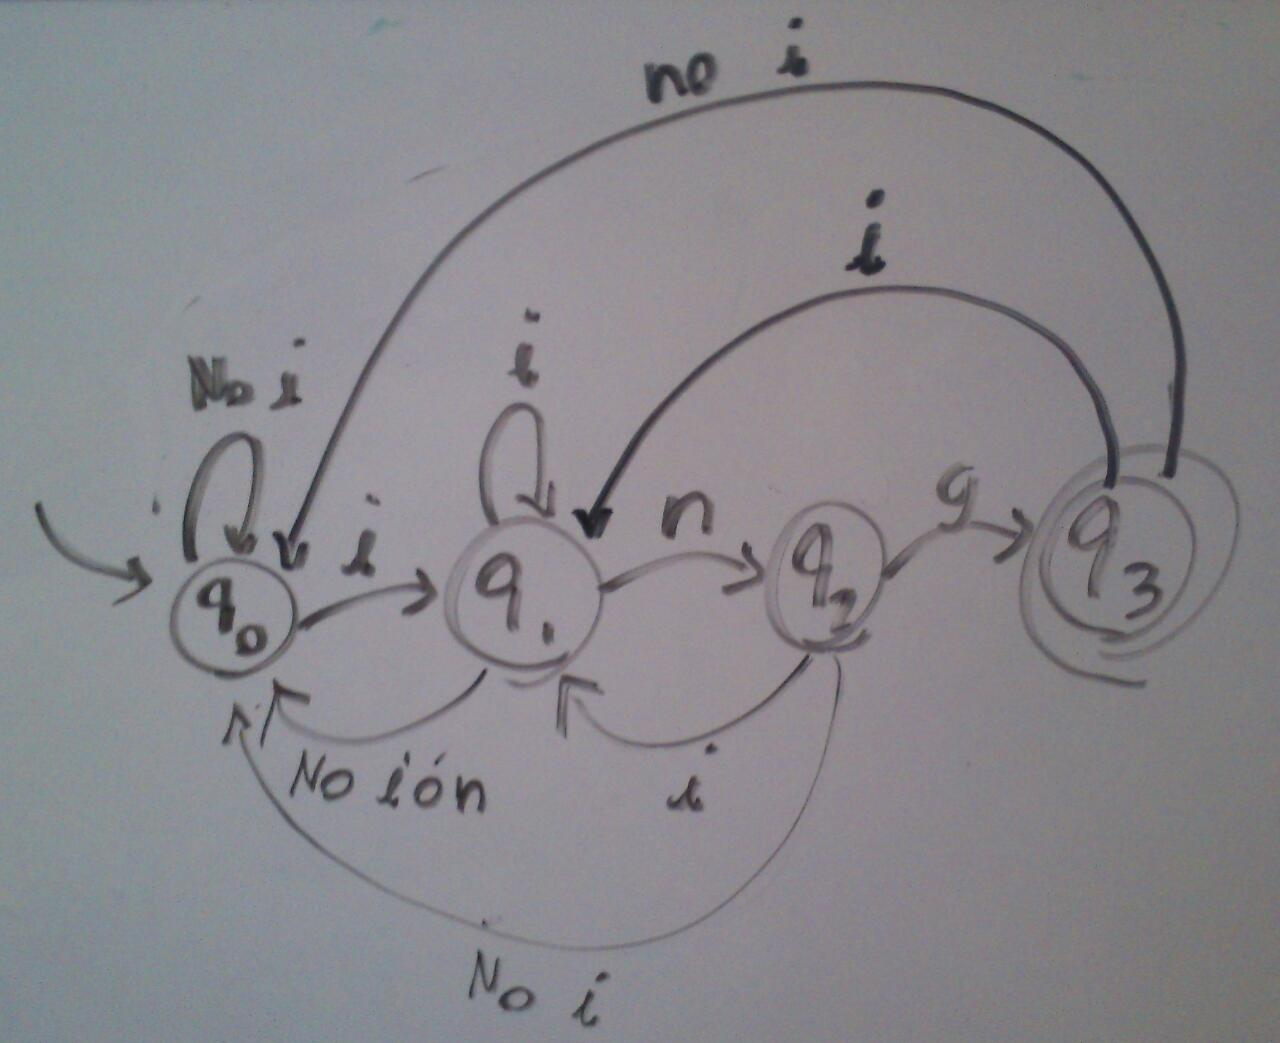
\includegraphics[width=0.7\textwidth]{diagrama.jpeg}\\
Cuya función de transición se describe con la siguiente tabla:\\
\begin{table}[H]
    \centering
        \begin{tabular}{|l |l |l |l |l}        
        \hline
        \textbf{$\delta$} & \textbf{No i} & \textbf{i} & \textbf{n} \textbf{g} \\
        \hline
        \textbf{$\rightarrow$q0} & q0 & q1 & $\emptyset$ & $\emptyset$ \\
        \hline
        \textbf{q1} & q0 & q1 & q2 & q0 \\    
        \hline
        \textbf{q2} & q0 & q1 & q0 & q3 \\
        \hline        
	\textbf{*q3} & q0 & q1 & q0 & q0 \\
        \hline        
        \end{tabular}
    \caption{Función de transición para el automata}

\end{table}

\end{document}

